\documentclass[8pt]{beamer}\usepackage[]{graphicx}\usepackage[]{color}
%
% \def\expect#1#2{\underset{#1}{\mathbb{E}}\left[#2\right]}
% \def\sumn{\sum_{n=1}^N}
% \def\x{x}
% \def\xvec{X}
% \def\w{w}
% \def\onevec{1_N}
% \def\infl{\psi}

\usetheme{metropolis}           % Use metropolis theme
\usepackage{amsmath}
\usepackage{tikz}


% This file contains the boilerplate that knitr would put at the top of
% a knitr document if you ran knitr with \begin{document} ... \end{document}.
% By including it once in the main document, you can knit and \input{}
% Rnw files that contain only individual sections.

\usepackage[]{graphicx}
\usepackage[]{color}
%% maxwidth is the original width if it is less than linewidth
%% otherwise use linewidth (to make sure the graphics do not exceed the margin)
\makeatletter
\def\maxwidth{ %
  \ifdim\Gin@nat@width>\linewidth
    \linewidth
  \else
    \Gin@nat@width
  \fi
}
\makeatother

\definecolor{fgcolor}{rgb}{0.345, 0.345, 0.345}
\newcommand{\hlnum}[1]{\textcolor[rgb]{0.686,0.059,0.569}{#1}}%
\newcommand{\hlstr}[1]{\textcolor[rgb]{0.192,0.494,0.8}{#1}}%
\newcommand{\hlcom}[1]{\textcolor[rgb]{0.678,0.584,0.686}{\textit{#1}}}%
\newcommand{\hlopt}[1]{\textcolor[rgb]{0,0,0}{#1}}%
\newcommand{\hlstd}[1]{\textcolor[rgb]{0.345,0.345,0.345}{#1}}%
\newcommand{\hlkwa}[1]{\textcolor[rgb]{0.161,0.373,0.58}{\textbf{#1}}}%
\newcommand{\hlkwb}[1]{\textcolor[rgb]{0.69,0.353,0.396}{#1}}%
\newcommand{\hlkwc}[1]{\textcolor[rgb]{0.333,0.667,0.333}{#1}}%
\newcommand{\hlkwd}[1]{\textcolor[rgb]{0.737,0.353,0.396}{\textbf{#1}}}%
\let\hlipl\hlkwb

\usepackage{framed}
\makeatletter
\newenvironment{kframe}{%
 \def\at@end@of@kframe{}%
 \ifinner\ifhmode%
  \def\at@end@of@kframe{\end{minipage}}%
  \begin{minipage}{\columnwidth}%
 \fi\fi%
 \def\FrameCommand##1{\hskip\@totalleftmargin \hskip-\fboxsep
 \colorbox{shadecolor}{##1}\hskip-\fboxsep
     % There is no \\@totalrightmargin, so:
     \hskip-\linewidth \hskip-\@totalleftmargin \hskip\columnwidth}%
 \MakeFramed {\advance\hsize-\width
   \@totalleftmargin\z@ \linewidth\hsize
   \@setminipage}}%
 {\par\unskip\endMakeFramed%
 \at@end@of@kframe}
\makeatother

\definecolor{shadecolor}{rgb}{.97, .97, .97}
\definecolor{messagecolor}{rgb}{0, 0, 0}
\definecolor{warningcolor}{rgb}{1, 0, 1}
\definecolor{errorcolor}{rgb}{1, 0, 0}
\newenvironment{knitrout}{}{} % an empty environment to be redefined in TeX

\usepackage{alltt}

%%%%%%%%%%%%%%%%%%%%%%%%%%%%%%%%%%%%%%
%%%%%%%%%%%%%%%%%%%%%%%%%%%%%%%%%%%%%%
% Do not edit the TeX file your work
% will be overwritten.  Edit the RnW
% file instead.
%%%%%%%%%%%%%%%%%%%%%%%%%%%%%%%%%%%%%%
%%%%%%%%%%%%%%%%%%%%%%%%%%%%%%%%%%%%%%





%%%%%%%%%%%%%%%%%%%%%%
%%%%%%%%%%%%%%%%%%%%%%
%%%%%%%%%%%%%%%%%%%%%%
% Plots

\newcommand{\BaseHistogram}{
\begin{knitrout}
\definecolor{shadecolor}{rgb}{0.969, 0.969, 0.969}\color{fgcolor}

{\centering 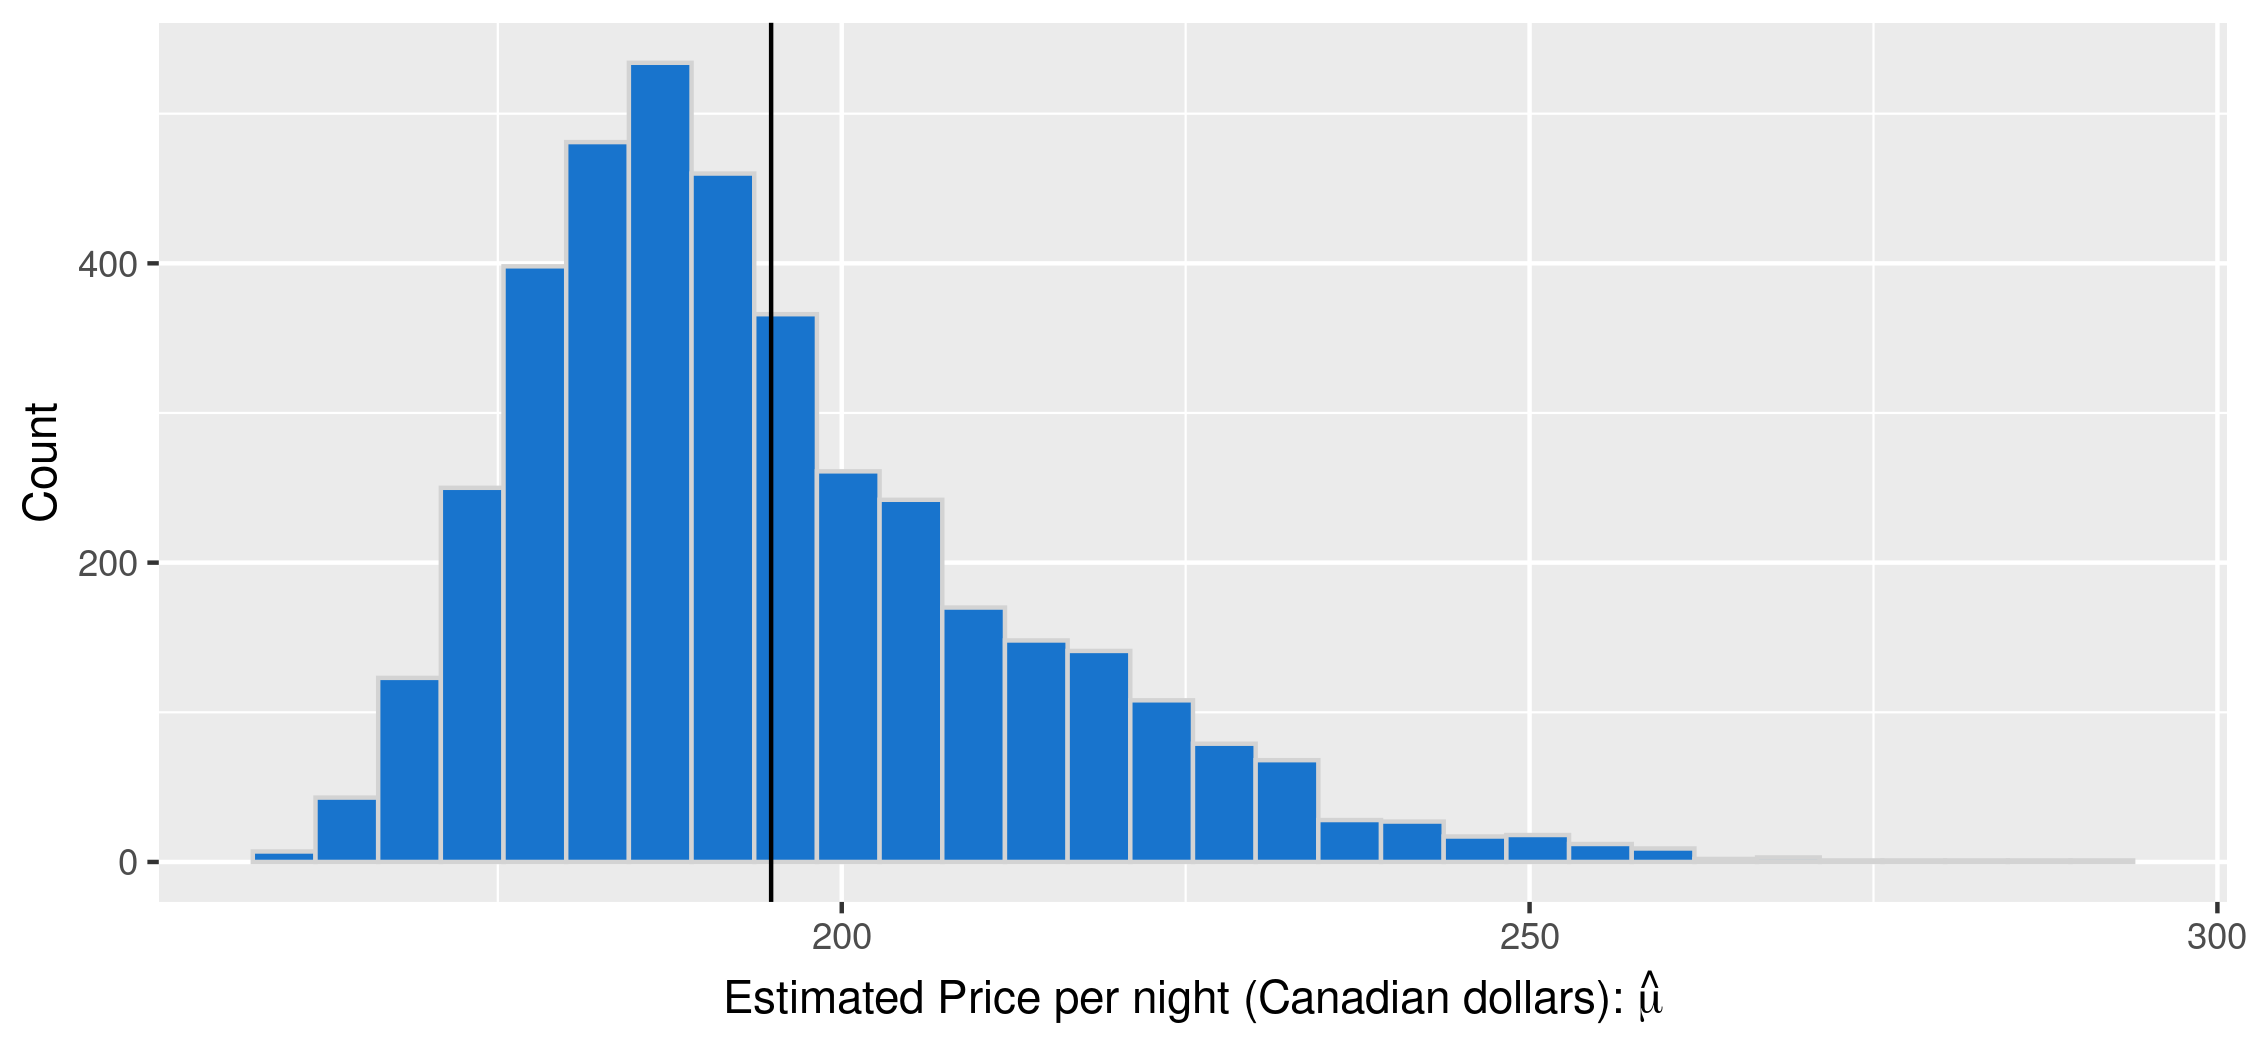
\includegraphics[width=0.98\linewidth,height=0.461\linewidth]{figure/base-hist-1} 

}



\end{knitrout}
}


\newcommand{\BaseHistogramWithArrow}{
\begin{knitrout}
\definecolor{shadecolor}{rgb}{0.969, 0.969, 0.969}\color{fgcolor}

{\centering 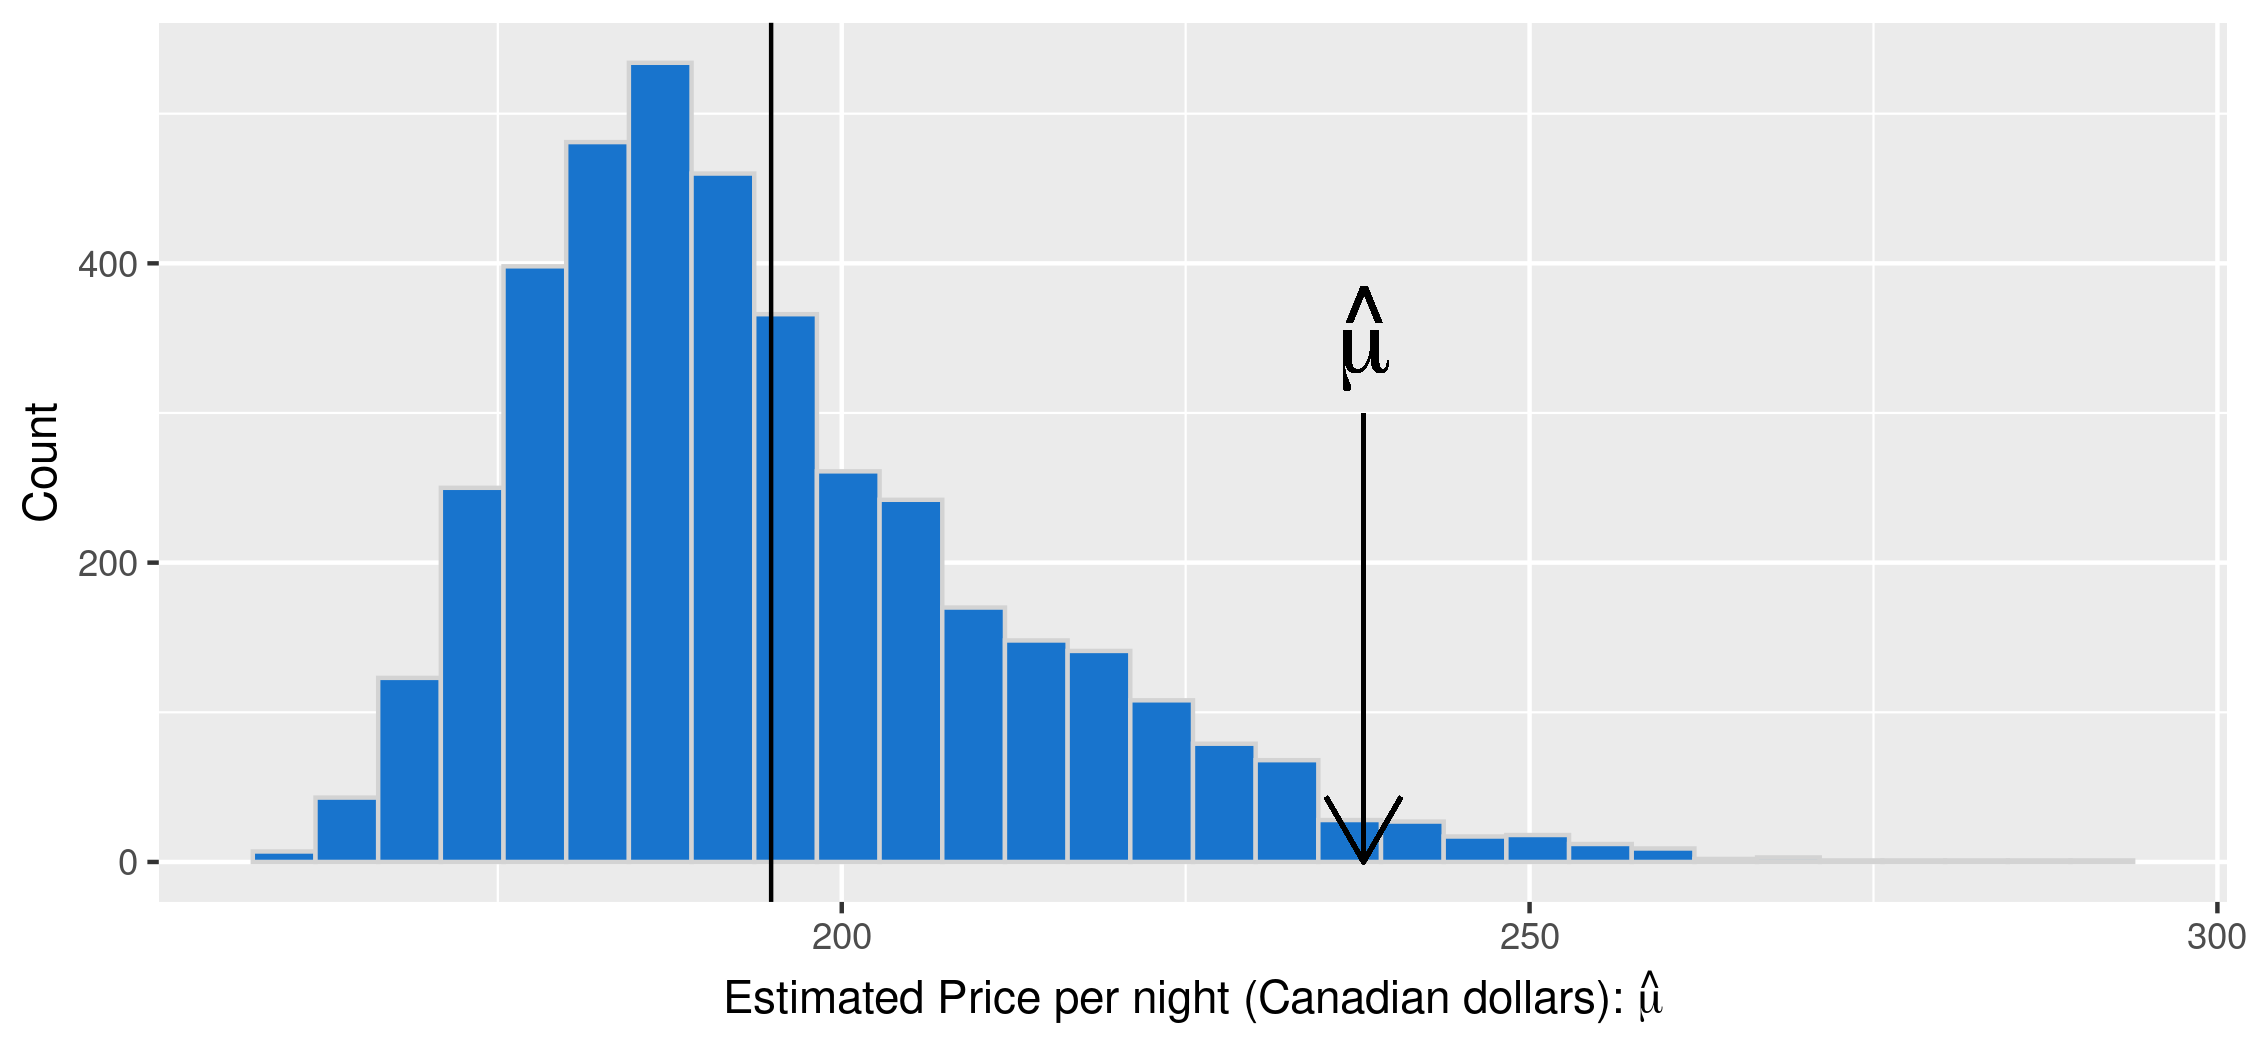
\includegraphics[width=0.98\linewidth,height=0.461\linewidth]{figure/base-hist-arrow-1} 

}



\end{knitrout}
}



\newcommand{\BaseHistogramFaded}{
\begin{knitrout}
\definecolor{shadecolor}{rgb}{0.969, 0.969, 0.969}\color{fgcolor}

{\centering 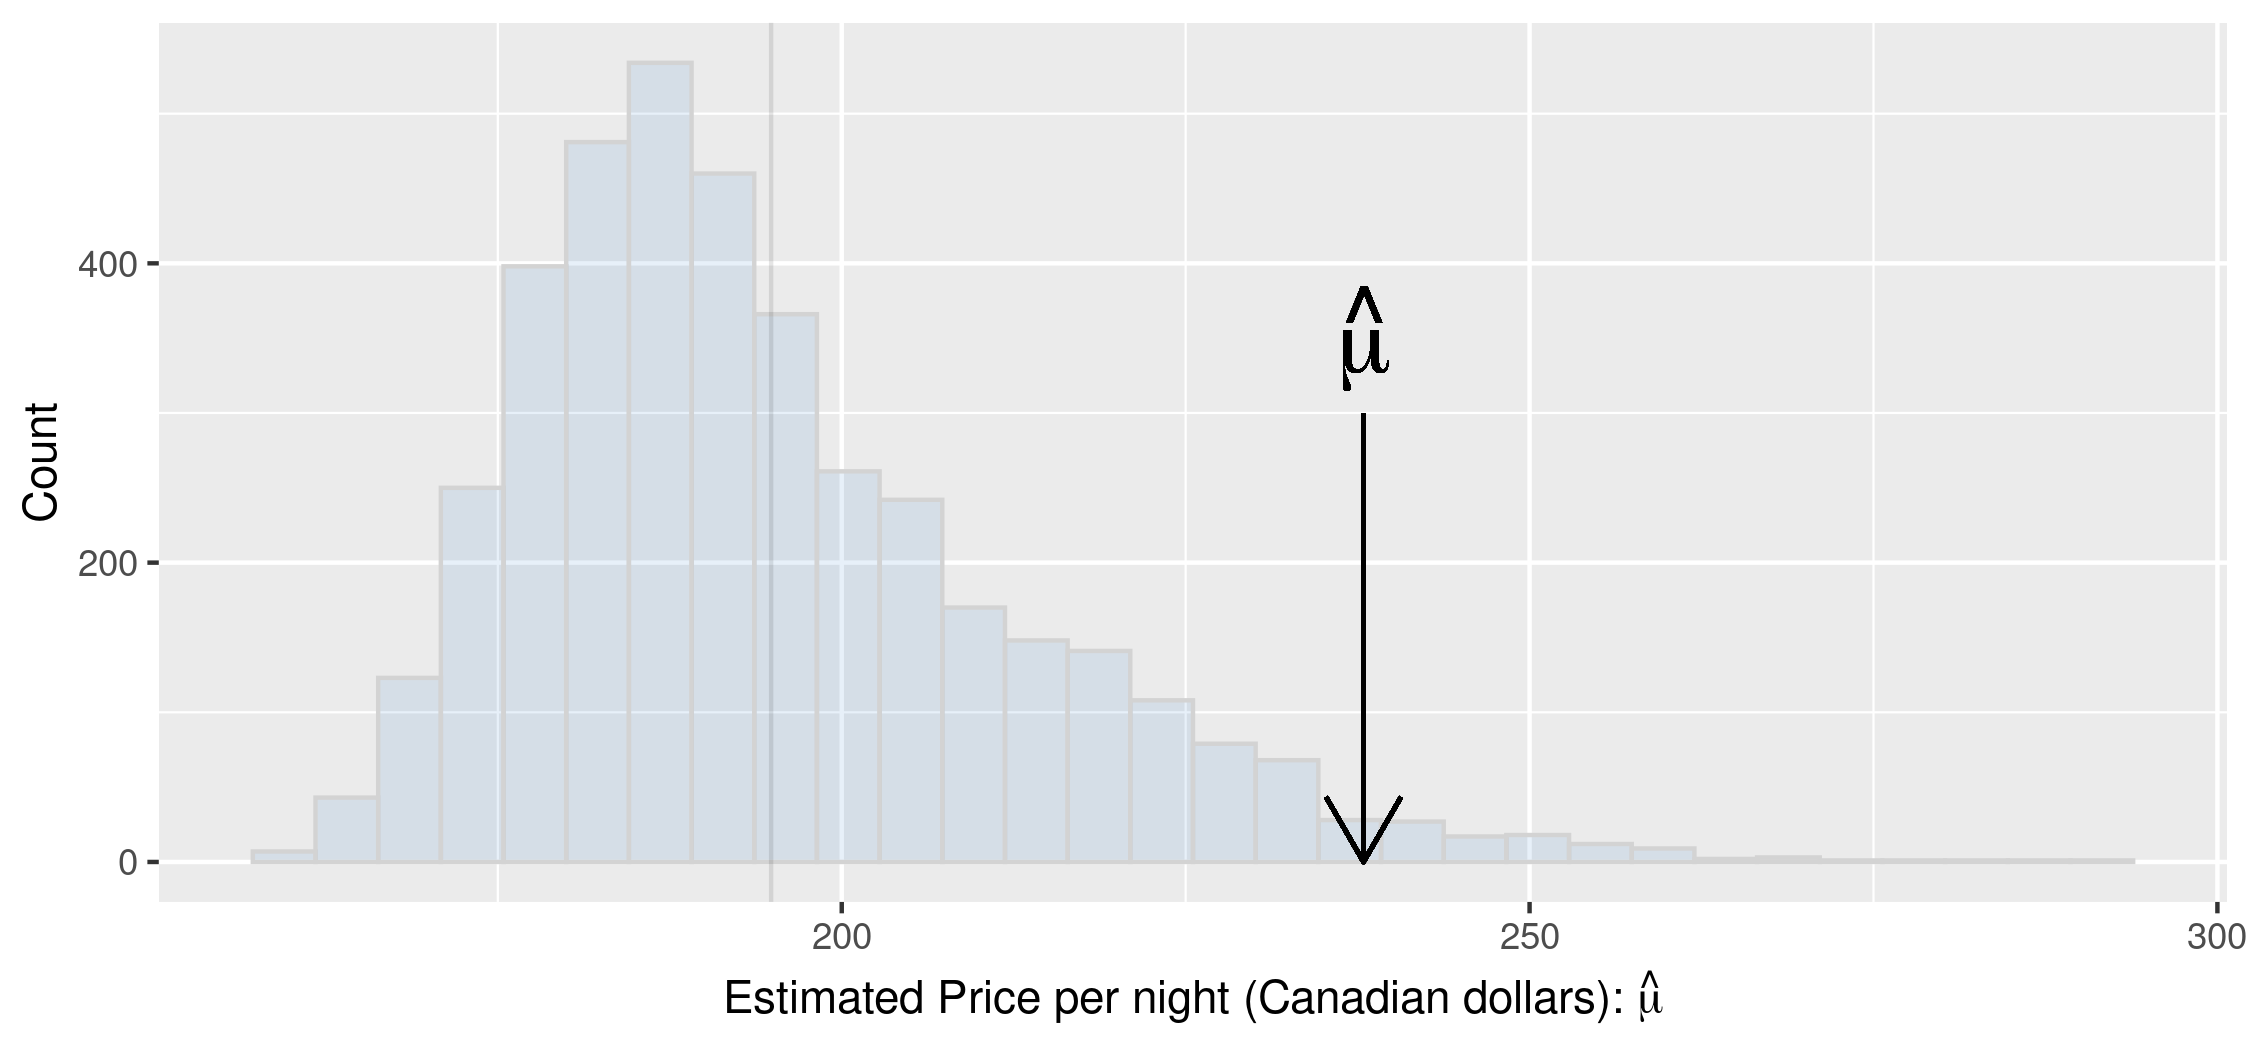
\includegraphics[width=0.98\linewidth,height=0.461\linewidth]{figure/base-hist-faded-1} 

}



\end{knitrout}
}


\newcommand{\SingleCI}{
\begin{knitrout}
\definecolor{shadecolor}{rgb}{0.969, 0.969, 0.969}\color{fgcolor}

{\centering 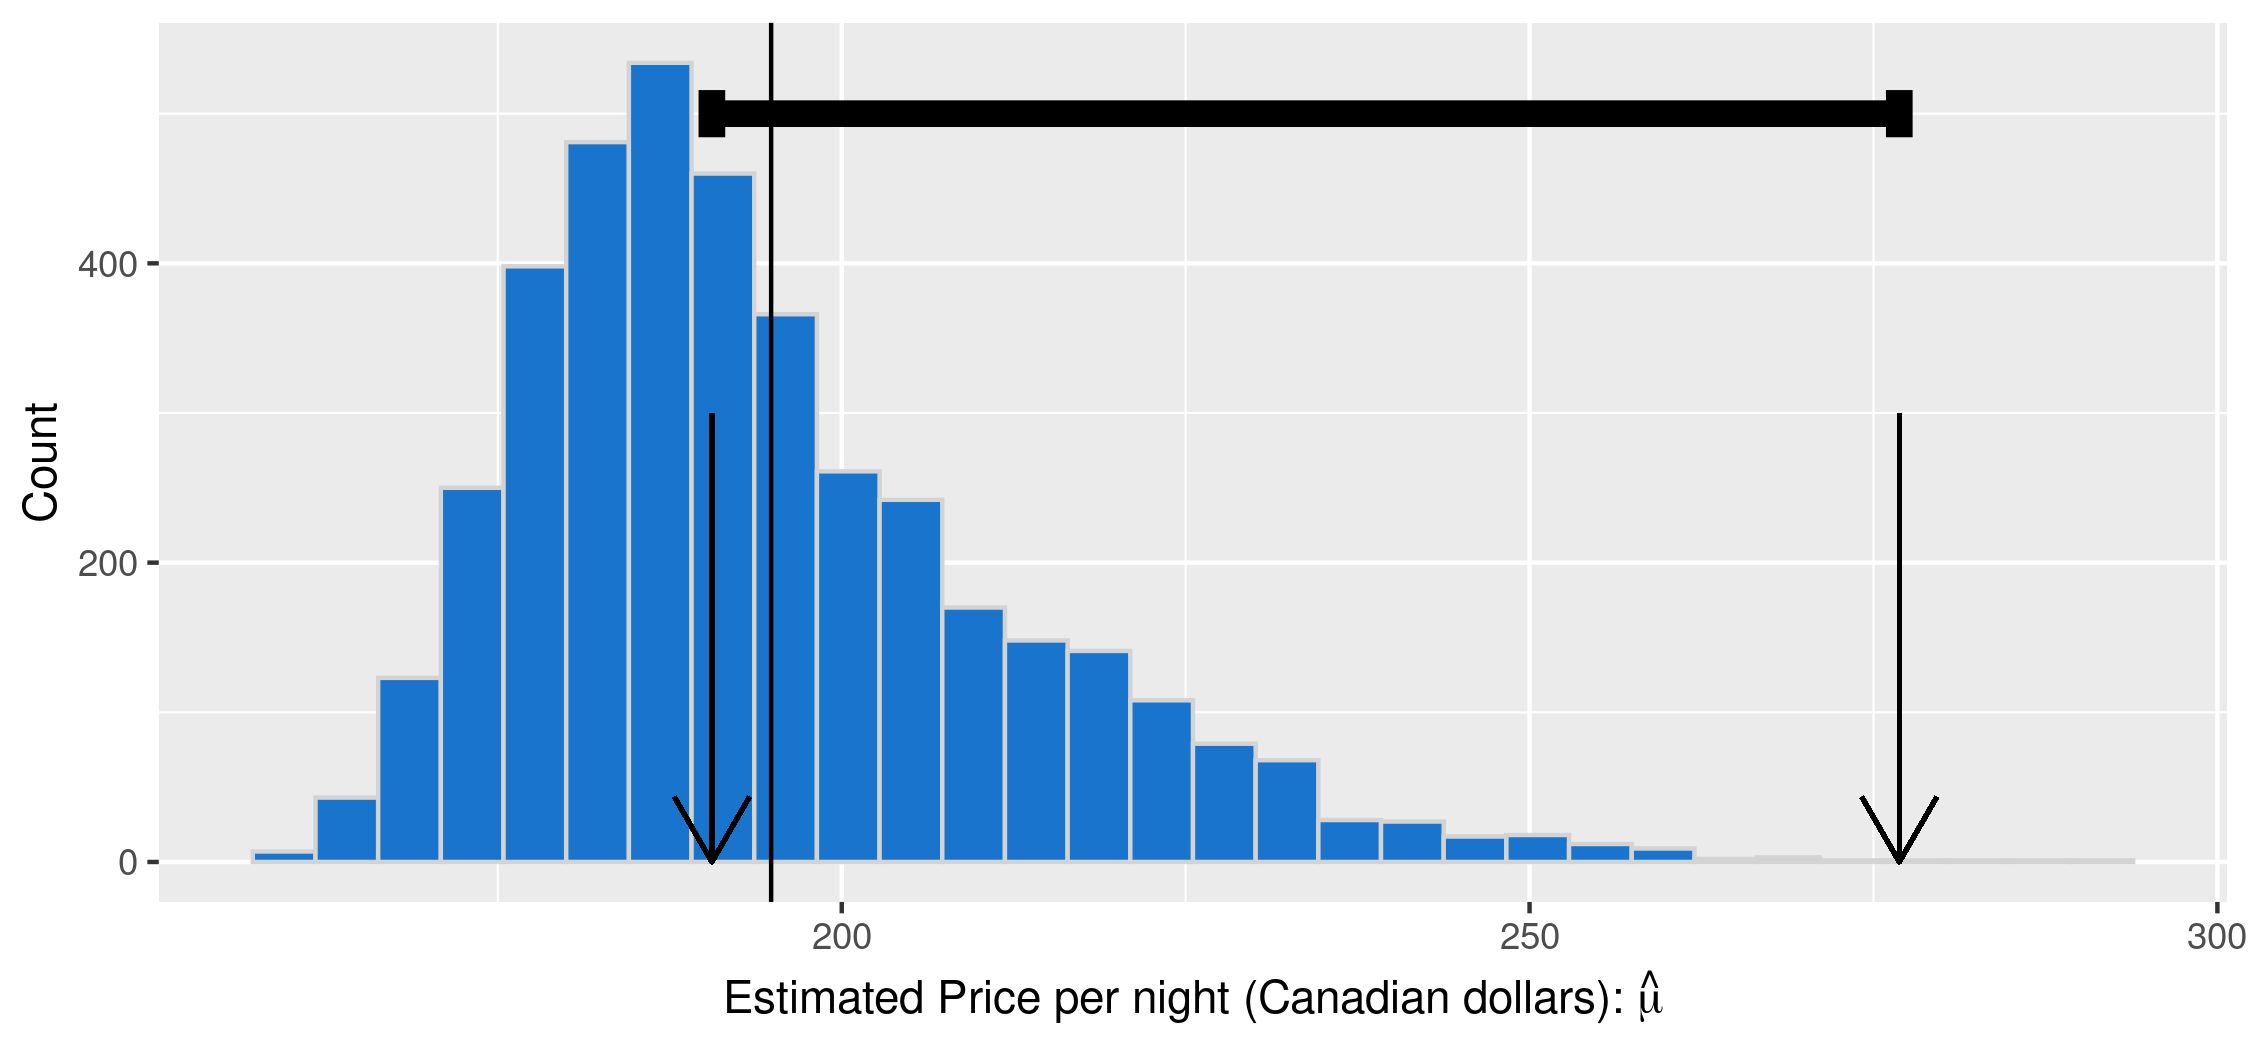
\includegraphics[width=0.98\linewidth,height=0.461\linewidth]{figure/base-hist-ci-1} 

}



\end{knitrout}
}




\newcommand{\SingleCIB}{
\begin{knitrout}
\definecolor{shadecolor}{rgb}{0.969, 0.969, 0.969}\color{fgcolor}

{\centering 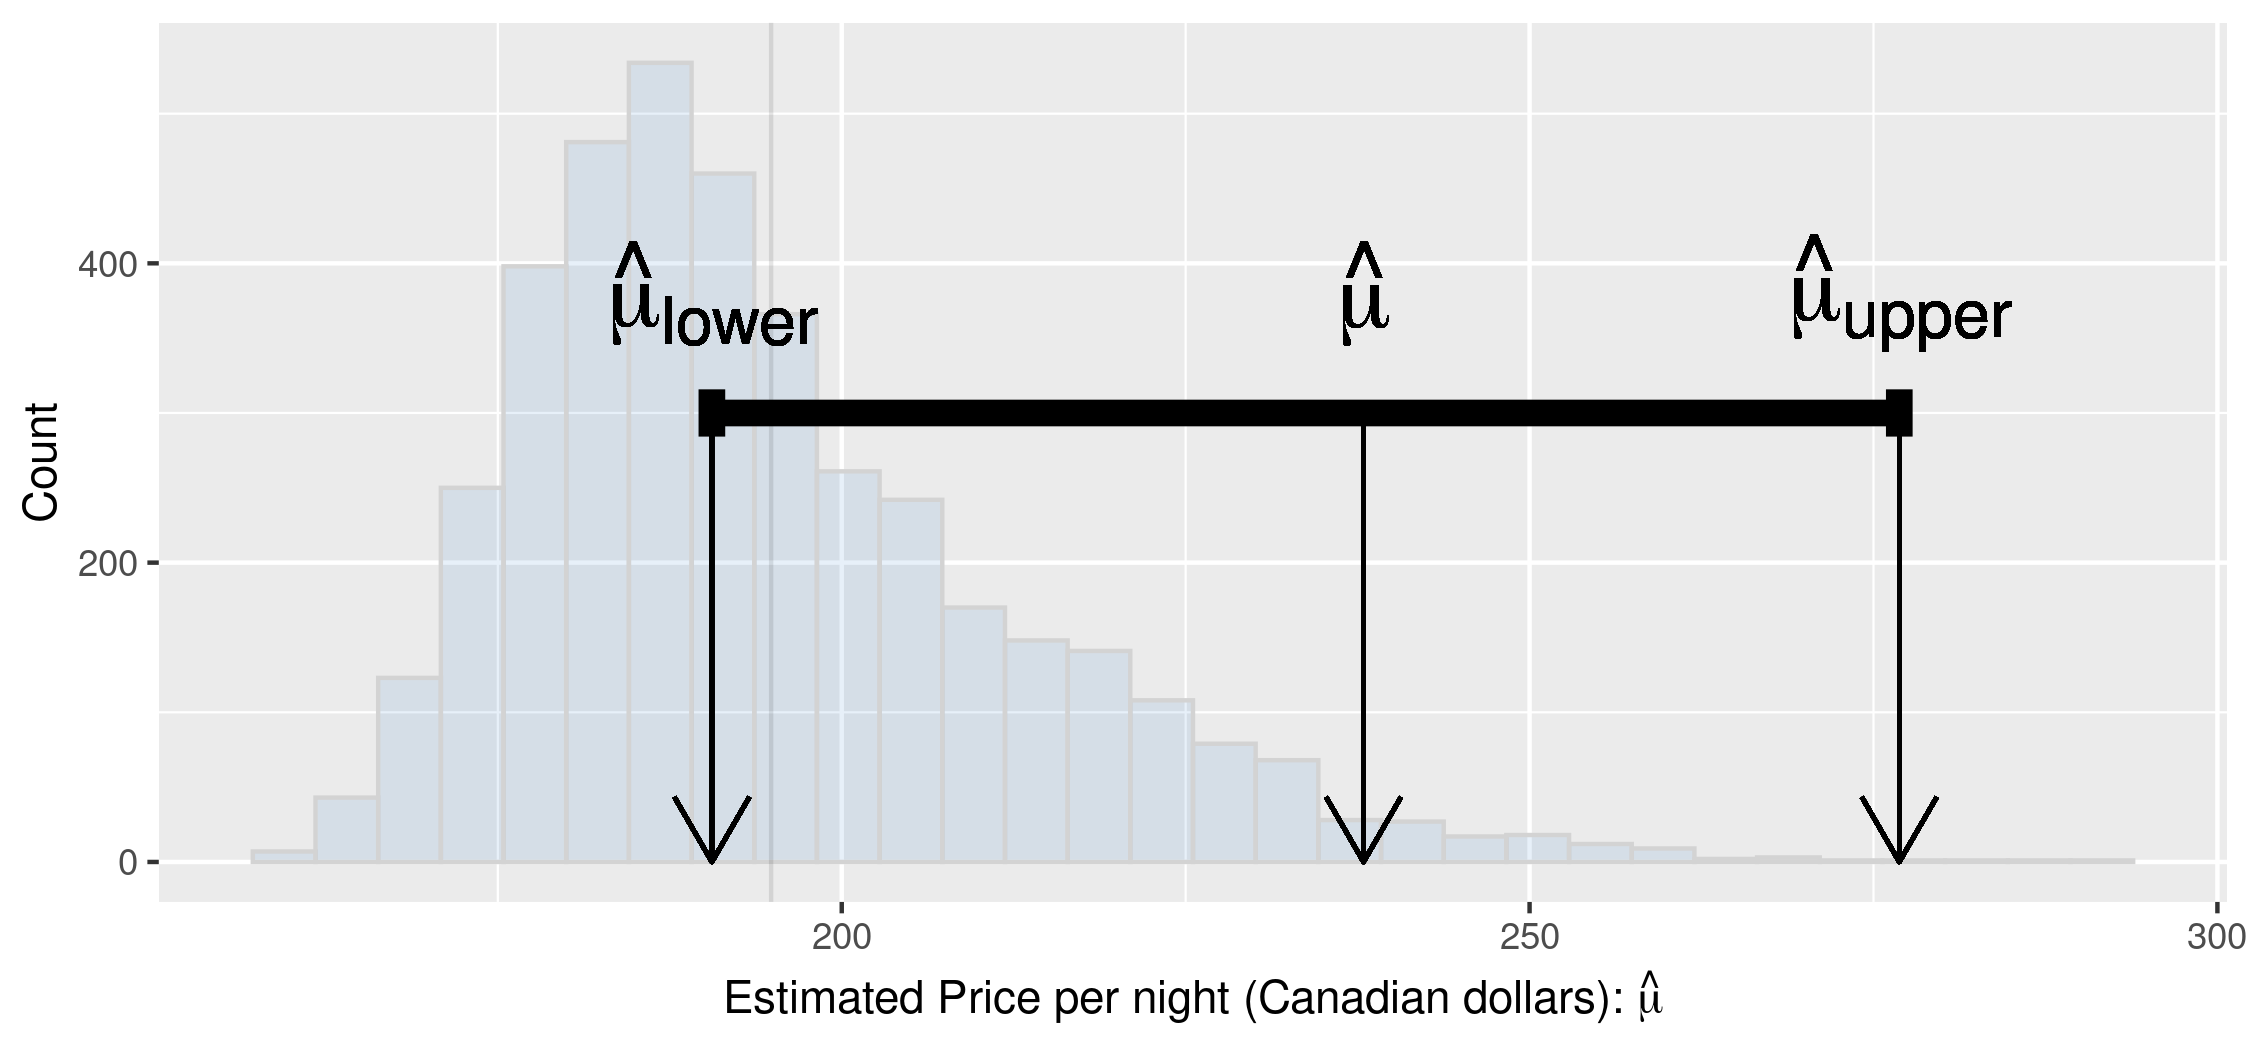
\includegraphics[width=0.98\linewidth,height=0.461\linewidth]{figure/base-hist-cib-1} 

}



\end{knitrout}
}



\newcommand{\MultipleCIs}{



\begin{knitrout}
\definecolor{shadecolor}{rgb}{0.969, 0.969, 0.969}\color{fgcolor}

{\centering 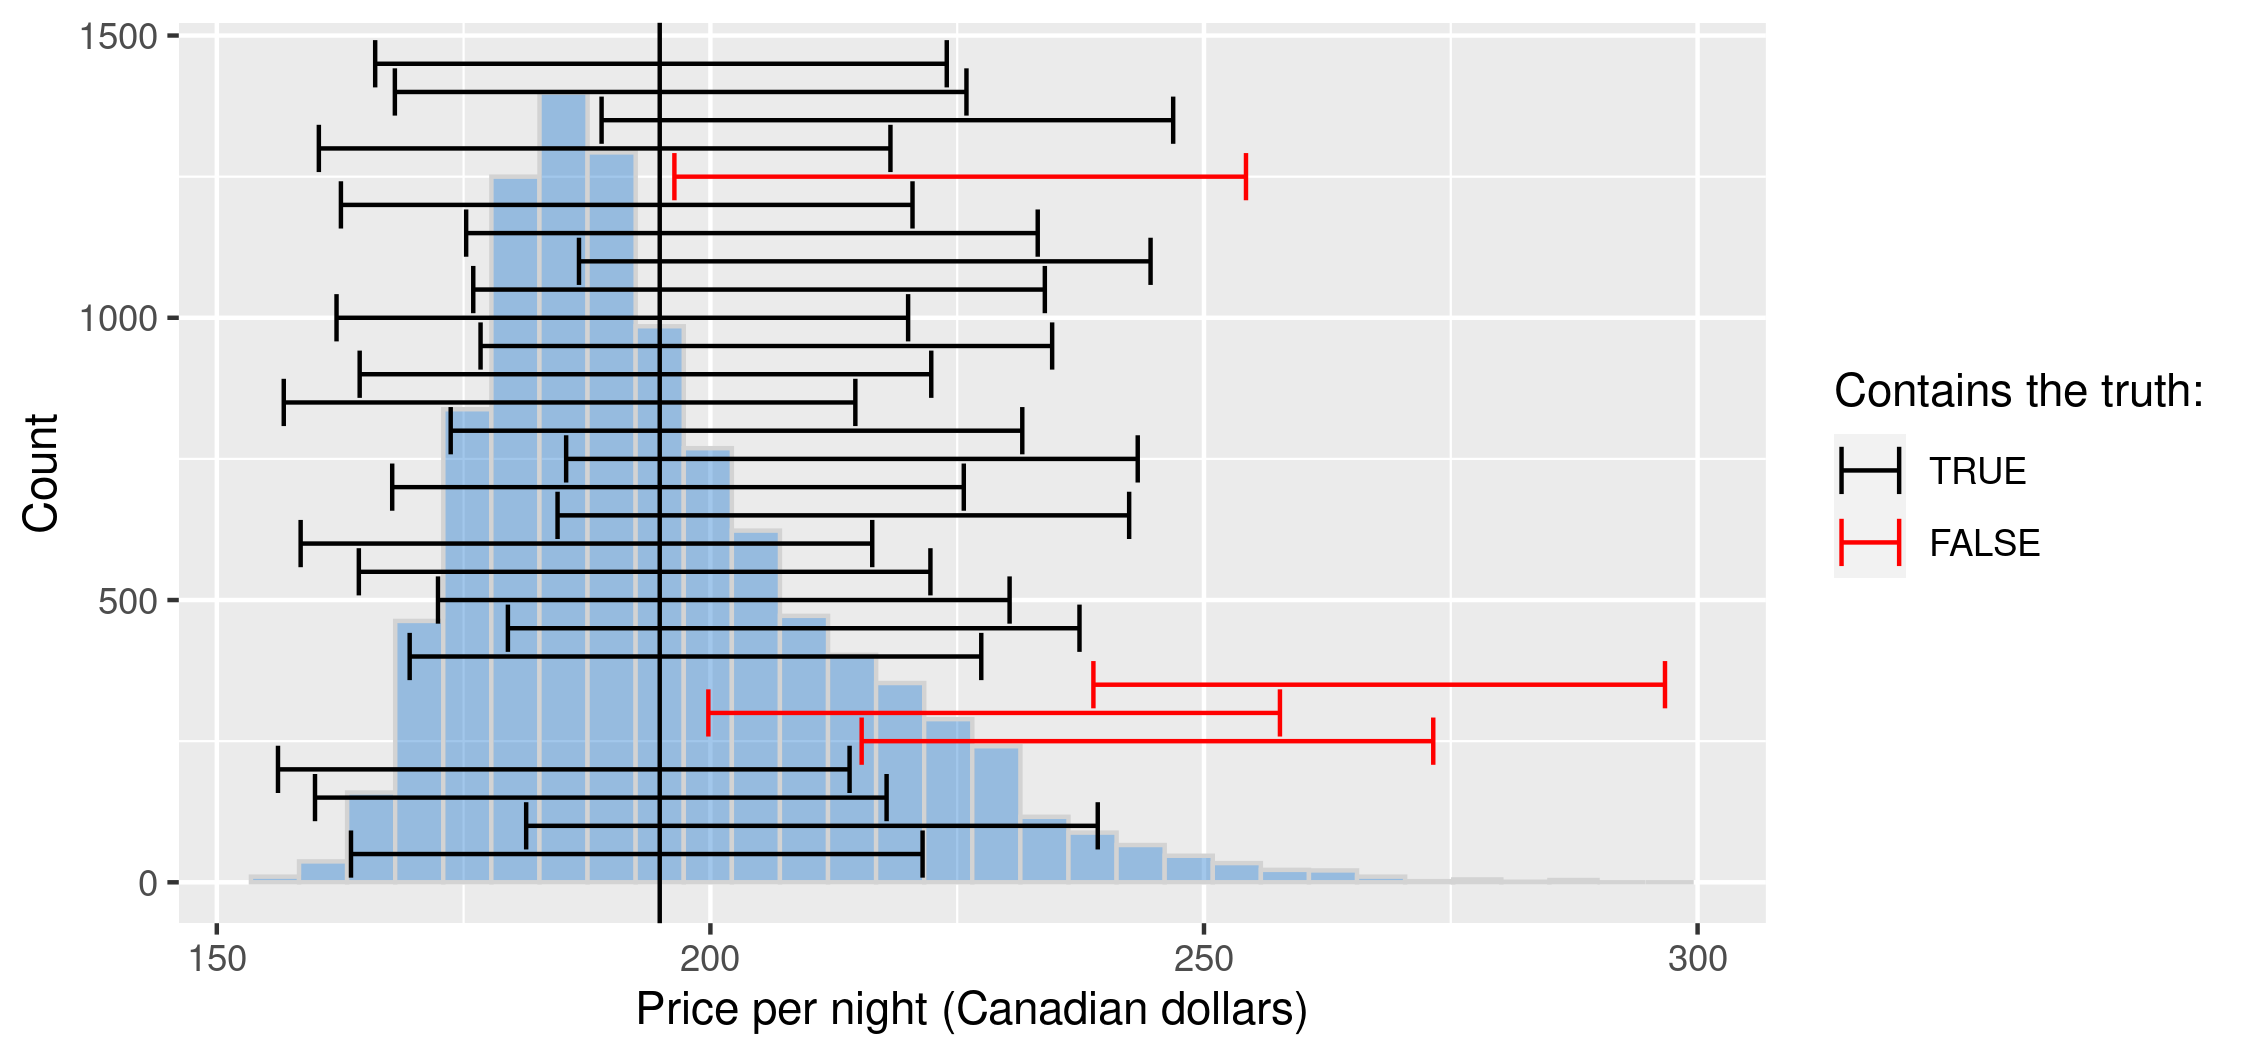
\includegraphics[width=0.98\linewidth,height=0.461\linewidth]{figure/base-hist-cis-1} 

}



\end{knitrout}
}


\usepackage{listings}
\lstset
{
    language=[LaTeX]TeX,
    breaklines=true,
    basicstyle=\tt\scriptsize,
    keywordstyle=\color{blue},
    identifierstyle=\color{magenta},
}

\title{CI introduction}
\author{Ryan Giordano}
\date{Dec 14th, 2021}
\institute{Massachusetts Institute of Technology}

\begin{document}



%%%%%%%%%%%%%%%%%%%%%%%%%%%%%%%%%%%%%%%%%%%%%%%%%%%%%%%%%%%%%%%%%%%%%%%
%%%%%%%%%%%%%%%%%%%%%%%%%%%%%%%%%%%%%%%%%%%%%%%%%%%%%%%%%%%%%%%%%%%%%%%
%%%%%%%%%%%%%%%%%%%%%%%%%%%%%%%%%%%%%%%%%%%%%%%%%%%%%%%%%%%%%%%%%%%%%%%

\begin{frame}[fragile]{Dataset}

Recall our running example from previous classes:\footnotemark[1]

\begin{itemize}
    \item We're interested in the mean price of AirBNBs in our city ($\mu$)
    \item We can't observe them all, so we take the mean
          price of a sample of 200 ($\hat\mu(X) = \frac{1}{200} \sum_{n=1}^{200} x_n$)
\end{itemize}

\onslide<4->{
\textbf{Key idea: }

Instead of a ``point estimate'' $\hat\mu(X)$,
estimate an interval $(\hat\mu_{lower}(X), \hat\mu_{upper}(X))$.
}

\begin{center}
\begin{minipage}{0.9\textwidth}
\only<1>{
\BaseHistogram{}
}
\only<2>{
\BaseHistogramWithArrow{}
}
\only<3>{
\BaseHistogramFaded{}
}
\only<4>{
\SingleCIB{}
}
\end{minipage}
\end{center}

\vfill
\footnotetext[1]{
Taken from Chapter 10 of ``Data Science: A First Introduction'' by
Timbers, Campbell, and Lee
\url{https://ubc-dsci.github.io/introduction-to-datascience/}
}

\end{frame}




%%%%%%%%%%%%%%%%%%%%%%%%%%%%%%%%%%%%%%%%%%%%%%%%%%%%%%%%%%%%%%%%%%%%%%%
%%%%%%%%%%%%%%%%%%%%%%%%%%%%%%%%%%%%%%%%%%%%%%%%%%%%%%%%%%%%%%%%%%%%%%%
%%%%%%%%%%%%%%%%%%%%%%%%%%%%%%%%%%%%%%%%%%%%%%%%%%%%%%%%%%%%%%%%%%%%%%%

\begin{frame}[t, fragile]{Dataset}

\textbf{Key idea: }

Instead of a ``point estimate'' $\hat\mu(X)$,
estimate an interval $(\hat\mu_{lower}(X), \hat\mu_{upper}(X))$.

\onslide<2->{

\textbf{We would like to choose our interval such that: }

$P(\mu \in (\hat\mu_{lower}(X), \hat\mu_{upper}(X))) \ge 0.9$

Such an interval is a \textbf{valid confidence interval} with a
\textbf{level} of 0.9.
}

% \onslide<5->{
% \textbf{Question: }
% Is $(-\infty, \infty)$ a valid confidence interval with level 0.9?
% }

\begin{center}
\begin{minipage}{0.9\textwidth}
% \only<1>{
% \SingleCIB{}
% }
\only<1->{
\MultipleCIs{}
}
\end{minipage}
\end{center}

\end{frame}



% %%%%%%%%%%%%%%%%%%%%%%
% \hrulefill
%
% Let's annotate this graphic using TikZ.
%
% \begin{lstlisting}
% \begin{center}
% \begin{minipage}{0.38\textwidth}
% 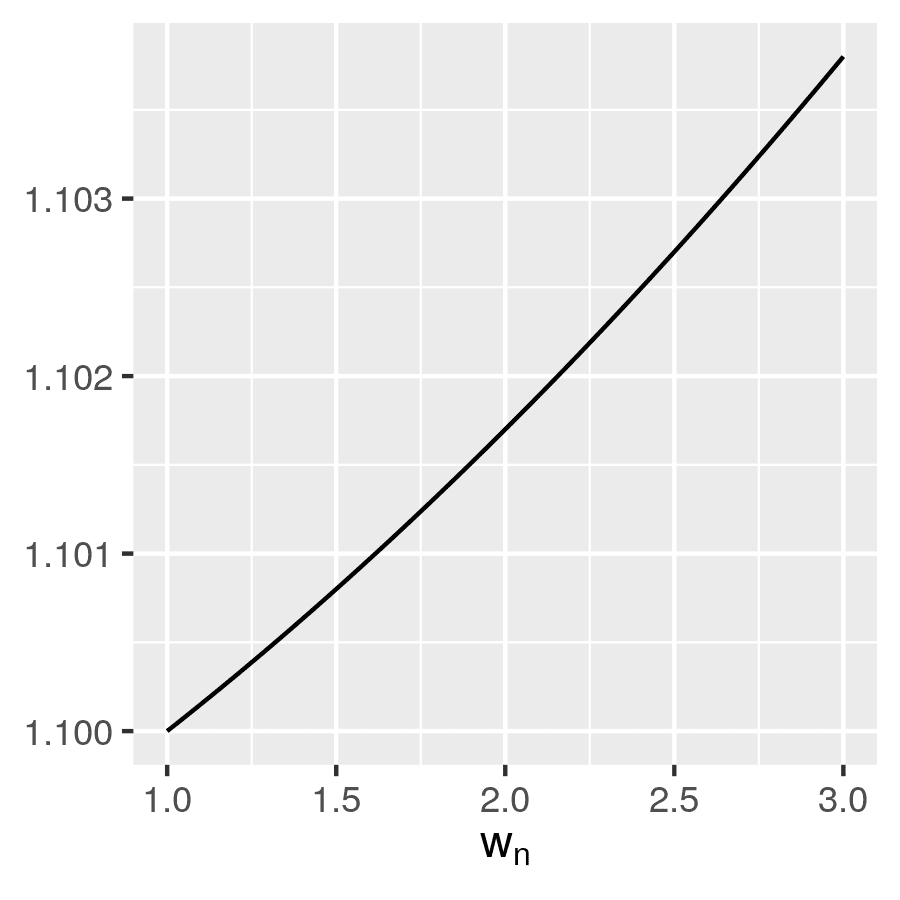
\includegraphics[width=\textwidth]{e_beta_w}
% \end{minipage}
% \end{center}
% \end{lstlisting}
%
% From now on, everything I'm going to do will be within the minipage.


\end{document}
